\section{Prüfung der Vollständigkeit}

Von \cite{shanbhag2014optimizing} wurde die Vollständigkeit der Regelmenegen geprüft. Eine Regelmenge wird dann als vollständig gewertet, wenn sie genutzt werden kann, um einen Suchraum von allen kreuzproduktfreien Plänen aus einem initialen Plan, der keine Kreuzprodukte enthält, zu erzeugen. In diesem Zusammenhang lassen sich drei Aspekte genauer betrachteten: (1) alle Pläne müssen gefunden werden; (2) die Pläne müssen kreuzproduktfrei sein; (3) sie müssen aus einem initialen Plan ohne Kreuzprodukte gebildet werden.

Um sicherzustellen, dass die erzeugten Pläne kreuproduktfrei sind, wurde von \cite{shanbhag2014optimizing} ein Mechanismus zur Kreuzproduktunterdrückung implementiert. Der Mechanismus sieht vor, dass nachdem ein neuer Plan mit Hilfe einer Regel erzeugt wurde, geprüft wird ob der erzeugte Plan kreuzproduktfrei ist. Nur wenn das der Fall ist wird der neue Plan gespeichert. Falls der neue Plan Kreuzprodukte enthält, wird die Regel zwar als ausgeführt markiert, aber das Ergebnis nicht gespeichert. Nur Ergebnisse, die kreuzproduktfrei sind, werden als Input für eine Regel akzeptiert. Regelmengen, die Kreuzprodukte durch diesen Mechnanismus verhindern,  werden mit dem Postfix -CPS versehen. So entstehen die neuen Regelmengen RS-B0-CPS, RS-B1-CPS und RS-B2-CPS.





\subsection{Prüfung von Regelmenge RS-B0-CPS und RS-B1-CPS}

Bei der Prüfung der beiden Regelmengen RS-B0-CPS und RS-B1-CPS auf Voll\-ständigkeit wurde zuerst festgestellt, dass wenn RS-B1-CPS vollständig ist auch automatisch RS-B0-CPS als vollständig gilt. Dies lässt sich darauf zurückführen, dass im Gegensatz zu RS-B1-CPS die Regelmenge RS-B0-CPS eine weitere, zusätzliche Regel implementiert. Da bereits die Regelmenge RS-B1-CPS vollständig ist, ist auch automatisch die Regel RS-B0-CPS vollständig, da die zusätzliche Regel keine bisher unbekannten Pläne erzeugen kann.

In einem ersten Schritt wird gezeigt, dass für jeden Join-Graphen ein kreuzprodukfreier links-tiefer Baum erzeugt werden kann. 
Aus einem gegebenenen Join-Graphen $G = (V, E)$ kann ein links-tiefer Baum gebildet werden, indem ein belibiger Knoten $v \in V$ als Start-Teilbaum $T_1$ gewählt wird. Aus dem $G$ wird dann ein beliebiger Knoten ausgewählt, der mit einem Knoten aus $T_i$ über eine Kante $e \in E$ verbunden ist, aber nicht Teil von $T_i$. Dieser Knoten wird dann mit dem Teilbaum $T_i$ verknüpft, so dass ein neuer Teilbaum entsteht. Sobald alle Knoten $V$ Teil des Teilbaums sind, ist ein kreuzproduktfreier Baum gebildet.




\newtheorem{lem}{Lemma} 
\newtheorem{teo}{Theorem}
\begin{lem}
Gegeben sei ein kreuzproduktfreier Baum mit den Relationen $R_1, R_2, ... , R_k$. Mit Hilfe von RS-B1-CPS kann dieser Baum so transformiert werden, dass $T \Join R_k$ entsteht, wobei $T$ ein Join-Tree ist, der aus den Relationen $R_1, .., R_{k-1}$ zusammengesetzt ist.
\end{lem}


\begin{figure}[ht]
  \centering
  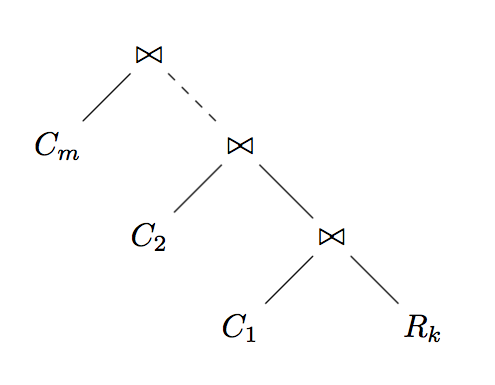
\includegraphics[scale=0.4]{03_Regeln/00_media/ReducedQueryTree.png}
  \caption{Reduzierter Query-Tree}
  \label{ReducedQueryTree}
\end{figure}



$Beweis:$ Das Ziel des Lemma ist es zu zeigen, dass aus einem gegebenen kreuzproduktfreien Baum die Relation mit der höchsten Nummer ($R_k$) so nach oben verschoben werden kann, dass diese Relation zuletzt gejoint wird.

Sei $R_k$ die Relation mit der höchsten nummer und die Relationen $R_1, ..., R_{k-1}$ andere Relationen innerhalb des Baums. Unter verwendung der Kummutativitätsregel können wir den gegebenen Query-Tree so transformieren, dass ein Baum entsteht, wie er in Abbildung \ref{ReducedQueryTree} zu sehen ist. $C_1, C_2, .. C_m$ sind hierbei Join Trees, die wiederum aus einer Menge von Relationen bestehen. Da die Anwendung von Kommutatvitität niemals ein Kreuzprodukt erzeugt, ist diese und alle zwischen Zustände des Graphen kreuzproduktfrei. Die in $m$ angegebene Zahl ist nicht nur die höchste Nummer mit der ein $C$ bezeichnet wird, sondern drückt zudem die Tiefe von $R_k$ aus.

\textbf{Basis Fall:} Bei einer Tiefe von $m = 1$, ist die Relation $R_k$ automatisch die letzte Relation die gejoint wird. Daher ist das Lemma für diesen Fall korrekt.

\textbf{Induktion:} Angenommen Lemma 1 ist korrekt für $m <= j$. Sei die Tiefe von $R_k$ $m = j+1$. 

\begin{figure}[ht]
  \centering
  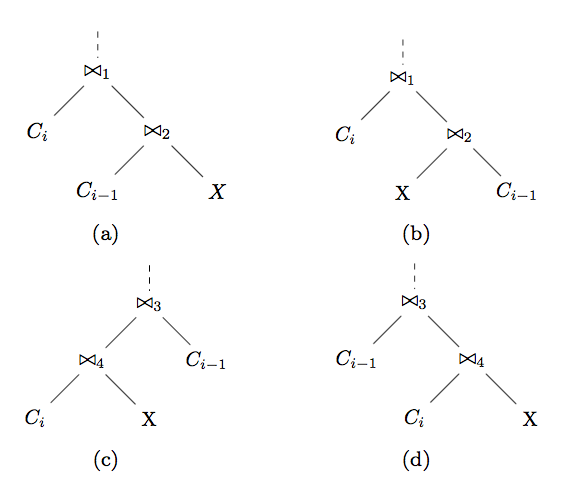
\includegraphics[scale=0.4]{03_Regeln/00_media/SwapC1.png}
  \caption{Tausch von $C_i$ und $C_{i-1}$}
  \label{SwapC1}
\end{figure}



Angenommen Lemma 1 sei korrekt für $ m <= j$ und die Tiefe von $R_k$ $m = j + 1$. Angenommen es existiert ein Subbaum aus $R_1, R_2,.. , R_k$. Solange $R_k$ die letzte Relation ist die gejoint wird, dann gibt es ein $C_1$ das jeoint werden kann mit mindestenens einem andereren der $C$ beispielsweie mit $C_i$. Dadurch ist es möglich, dass $C_i$ nach unten zu $C_1$ verschoben wird indem die folgende Sequenz an Regeln angewendet wird.

Wie in Abbildung \ref{SwapC1} a zu sehen ist, gibt es ein X, das die rechte Seite eines Subtrees darstellt und der mit $C_{i-1}$ gejoint ist. Wir wenden auf den Join $\Join_2$ die Kommutativitätsregel an, so entsteht Abbildung \ref{SwapC1} b. Auf den Join $\Join_1$ wird linke-Assoziativität angewendet, so entsteht $\Join_3$. Mit einer finalen Anwendung von Kommutativität auf $\Join_3$ entsteht \ref{SwapC1} d.

Jeder Zwischenschritt ist kreuzproduktfrei, da $C_i$ ein Join Prädikat mit $C_1$ besitzt welches Teil des Subtrees $X$  wie auch $C_{i-1}$.

Am Ende der Sequenz von Transformationen ist $C_i$ einen Schritt näher an $C_1$ gerückt. Jedes Mal, wenn die Sequenz angewendet wird, rückt $C_1$ noch ein Stück näher.

Zum Schnluss ist $C_1$ auf dem selben Level wie $C_i$ wie es in Abbildung \ref{} a zu sehen ist.  Mit Hilfe von linker Assoziativität kann dann der Baum aus Abbildung \ref{} b erzeugt werden.  Dieser Baum ist auch kreuzproduktfrei, da $C_i$ und $C_1$ ein gemeinsames Prädikat besitzen und so tuen es auch $R_k$ und $C_1$.

Die Tiefe von $R_k$ ist nun von $j + 1$ auf $j$ verkleinert, dies induziert, dass die Hypothese für $m <= j$ korrekt ist und somit das Lemma bewiesen.


\begin{lem}
Gegeben Sei ein Join-Graph $G$ und ein kreuzproduktfreier Query Tree, der aus G gebildet wurde, dann kann dieser in einen links-tiefen Tree basierend auf $G$ transformiert werden mit Hilfe von $RS-B1-CPS$.


\end{lem}

$Beweis:$ Angenommen die Relationen eines links-liefen Join-Trees sind nummeriert von $R_1$ bis $R_n$. Wie bereits zeigt in Lemma 1, ist die Transformation mit RS-B1-CPS möglich, die $R_n$ nach oben bewegt, sodass sie die letzte Relation ist, die gejoint wird. Die Regeln, die in RS-B1-CPS sind können angewendet werden, um den linken subTree des Resukatsbaums in einen Baum mit $R_{n-1}$ nach oben zu schieben. Es ist einfach zu zeigen, dass mit Hilfe von Indution, dass der gewünschte link-tiefe Baum erzeugt werden kann durch die Anwendung von RS-B1-CPS.

\begin{lem}
Gegeben sei ein Join Graph G. Ein beliebiger link-liefer Join Tree $T1$ kann in jeden kreuzproduktfrein Query Tree T2 transformiert werden mit RS-B1-CPS.
\end{lem}

$Beweis:$ Wie in Lemma 2 zu sehen, kann jeder Kreuzproduzktfreie Join Treee T2 in einen kreuzproduktfreien links-liefen Baum transfomriert werden. Wenn diese Sequenz, die zur Erzeugung des links-liefen baums ausgeführt wird, rückwärts abläuft, kann so der links-liefe Baum aus dem beliebigen Baum gebildet werden. Wobei anstatt von linker-Assoziativität rechte-Assoziativität zum Einsatz kommen muss. Zwar ist rechte-Assoziativität Teil nicht Teil von RS-B1-CPS kann jedoch mit Hilfe von Assoziativität und Kommutativität hergestellt werden. 
 

\begin{teo}
Die Regelmenge RS-B1-CPS ist vollständig, gegeben sei ein beliebiger kreuzproduktfreier Join Tree T1. dann ist es möglich alle anderen kreuzproduktfreien Bäume aus diesem zu erstellen, indem eine Reihe von Regeln als RS-B1-CPS angewendet werden.
\end{teo}

$Beweis:$ Der Bereis für die Vollständigkeit lässt sich aus Lemma 2 und Lemma 3 ableiten. Wir können jeden Tree in einen links-tiefen Baum umwnadeln und dies wieder 




Es wurde angenommen, dass für einen kreuzproduktfreien Baum mit den Relationen $R_1, R_2, ..., R_k$


\subsection{Unvollständigkeit von RS-B2}

\begin{figure}[ht]
  \centering
  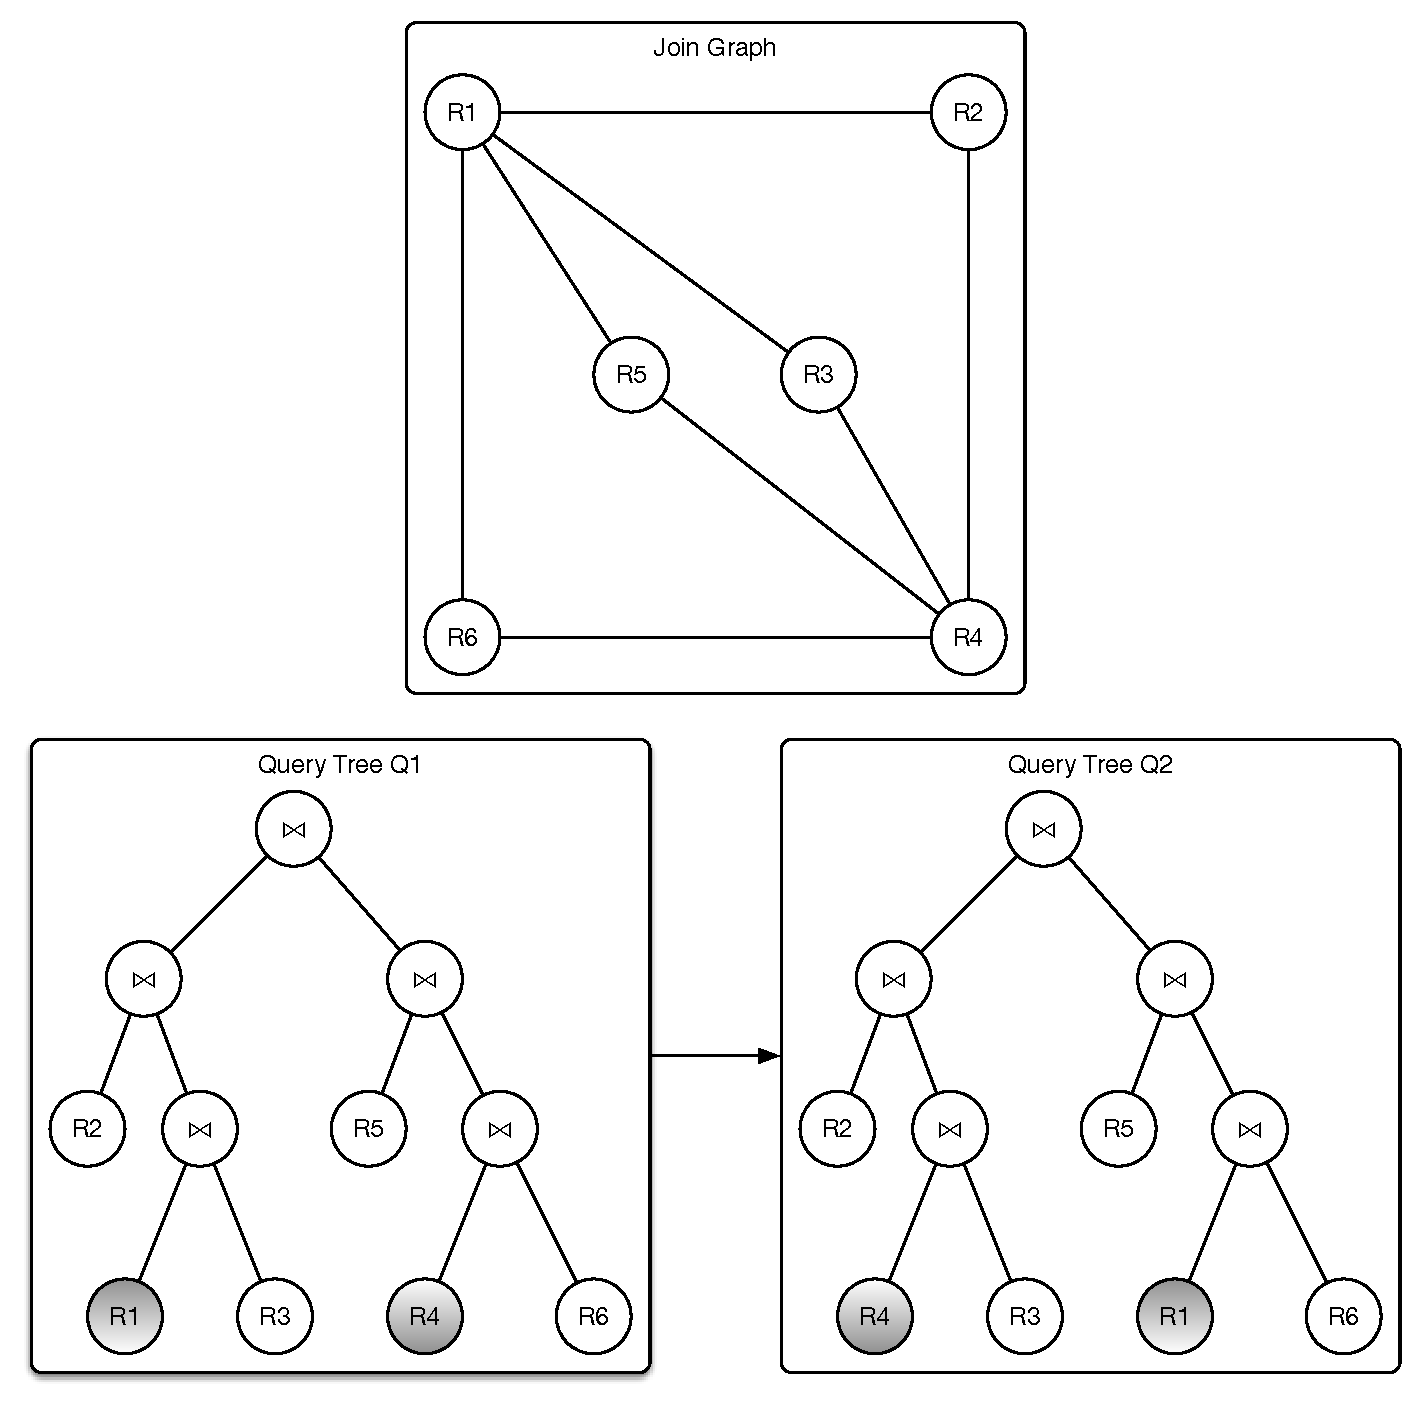
\includegraphics[width=\textwidth]{02_Related_Work/Graphs.pdf}
  \caption{Incompletness of RS-B2-CPS}
  \label{Incompleteness_RS-B2-CPS}
\end{figure}


Die Unvollständigkeit wurde mit Hilfe eines Beispiels belegt. Als Beispiel wurde der Bushy-Tree gewählt, der in Abbildung \ref{Incompleteness_RS-B2-CPS} zu sehen ist. Mit Hilfe der Regeln aus der Regelmenge RS-B2 sollte der initale Plan () in den Plan () umgewandelt werden. Dabei werden die vier Regeln der Regelmenge angewendet.

\begin{itemize}
\item Mit der Kommutativitätsregel ist es möglich ein Spiegelbild des original Baums herzustellen, aber nicht den Plan grundlegend zu verändern.
\item Bei der Anwendung von linker Assoziativität auf den Root-Knoten des Baum würde ein neuer Baum erzeugt werden dessen
\item Das Ergebnis von rechter Assoziativität ist symmetrisch zu linker Assoziativität.
\end{itemize}


Welche Regel auch immer auf den Baum angewendet wird, es ist nicht möglich den einen in den anderen Baum zu transformieren.

\subsection{Unvollständigkeit von RS-B2 mit Hilfe von PyroJ}

Mit Hilfe des Optimierers PyroJ - sein Aufbau wird in \ref{sec:pyroJ} behandelt - wurden die Regelsets ebenfalls auf ihre Vollständigkeit hin geprüft. Es wurde angenommen, dass zwei Ergebnismengen dann gleich sind, wenn die Anzahl der Äquivalenzklassen und die Anzahl der Operatorknoten gleich ist. Da wie zuvor festgestellt RS-B1 vollständig ist, wurde RS-B1 als Benchmark für andere Regelsets genutzt. Als Test-Case wurden Starqueries verwendet. Wie in Tabelle \ref{} zu sehen ist, wurde mit Hilfe von RS-B2 erheblich weniger Operatoren-Knoten erzeugt als mit RS-B1. \cite{} schlisst daher darauf, dass RS-B2 unvollständig ist.

Ebenfalls stellt \cite{} hervor, dass eine bestimmte Anfrage (Anfrage 7 des TPC-DS Benchmarks) bei der Nutzung des RS-B2 eine um 1.86 höher geschätzte Kosten als RS-B1 verursacht hatte.



\subsection{Hinweise auf Unvollständigkeit}